% Detailed User Flow Diagram with NLP Components Highlighted
% Requires: \usepackage{tikz}
% Shows both user actions and system processes

\begin{figure}[h]
\centering
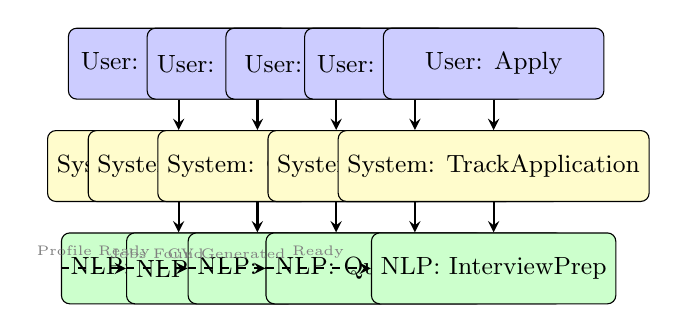
\begin{tikzpicture}[
    node distance = 1cm and 1.5cm,
    auto,
    user/.style = {
        rectangle,
        rounded corners = 3pt,
        minimum width = 2.8cm,
        minimum height = 0.9cm,
        text centered,
        draw = black,
        fill = blue!20,
        font = \small
    },
    system/.style = {
        rectangle,
        rounded corners = 3pt,
        minimum width = 2.8cm,
        minimum height = 0.9cm,
        text centered,
        draw = black,
        fill = yellow!20,
        font = \small
    },
    nlp/.style = {
        rectangle,
        rounded corners = 3pt,
        minimum width = 2.8cm,
        minimum height = 0.9cm,
        text centered,
        draw = black,
        fill = green!20,
        font = \small
    },
    arrow/.style = {
        ->,
        >=stealth,
        thick
    },
    label/.style = {
        font = \tiny,
        text = gray
    }
]

    % User actions (top row)
    \node [user] (u1) {User: Upload CV};
    \node [user, right of = u1] (u2) {User: Search Jobs};
    \node [user, right of = u2] (u3) {User: Select Job};
    \node [user, right of = u3] (u4) {User: Review CV};
    \node [user, right of = u4] (u5) {User: Apply};
    
    % System processes (middle row)
    \node [system, below of = u1, yshift = -0.3cm] (s1) {System: Extract Text};
    \node [system, below of = u2, yshift = -0.3cm] (s2) {System: Query\\Enhancement};
    \node [system, below of = u3, yshift = -0.3cm] (s3) {System: Generate\\Tailored CV};
    \node [system, below of = u4, yshift = -0.3cm] (s4) {System: Validate\\Quality};
    \node [system, below of = u5, yshift = -0.3cm] (s5) {System: Track\\Application};
    
    % NLP components (bottom row)
    \node [nlp, below of = s1, yshift = -0.3cm] (n1) {NLP: LLM Parsing};
    \node [nlp, below of = s2, yshift = -0.3cm] (n2) {NLP: Semantic\\Search};
    \node [nlp, below of = s3, yshift = -0.3cm] (n3) {NLP: Agentic\\Generation};
    \node [nlp, below of = s4, yshift = -0.3cm] (n4) {NLP: Quality\\Assessment};
    \node [nlp, below of = s5, yshift = -0.3cm] (n5) {NLP: Interview\\Prep};
    
    % Vertical connections
    \draw [arrow] (u1) -- (s1);
    \draw [arrow] (s1) -- (n1);
    \draw [arrow] (u2) -- (s2);
    \draw [arrow] (s2) -- (n2);
    \draw [arrow] (u3) -- (s3);
    \draw [arrow] (s3) -- (n3);
    \draw [arrow] (u4) -- (s4);
    \draw [arrow] (s4) -- (n4);
    \draw [arrow] (u5) -- (s5);
    \draw [arrow] (s5) -- (n5);
    
    % Horizontal flow
    \draw [arrow, dashed] (n1) -- node [label, above] {Profile Ready} (n2);
    \draw [arrow, dashed] (n2) -- node [label, above] {Jobs Found} (n3);
    \draw [arrow, dashed] (n3) -- node [label, above] {CV Generated} (n4);
    \draw [arrow, dashed] (n4) -- node [label, above] {Ready} (n5);
    
\end{tikzpicture}
\caption{Detailed User Flow with NLP Components}
\label{fig:user_flow_detailed}
\end{figure}

